%%%%%%%%%%%%%%%%%%%%%%%%%%%%%%%%%%%%%%%%%
% CU Boulder Physics Lab Writeup One Column
% LaTeX Template
% Version 1.0 (2022-10-05)
%
% This template has been downloaded from:
% http://www.LaTeXTemplates.com
%
% Original author:
% Mathias Legrand (legrand.mathias@gmail.com) titled Stylish Article 
% With extensive modifications by:
% Vel (vel@latextemplates.com)
% Further modifications for CU Boulder Physics by:
% Kristopher Bunker (kristopher.bunker@colorado.edu)
%
% License:
% CC BY-NC-SA 3.0 (http://creativecommons.org/licenses/by-nc-sa/3.0/)
%
%%%%%%%%%%%%%%%%%%%%%%%%%%%%%%%%%%%%%%%%%

%----------------------------------------------------------------------------------------
%	PACKAGES AND OTHER DOCUMENT CONFIGURATIONS
%----------------------------------------------------------------------------------------

\documentclass[10pt]{PhysLab1C} % Document font size

\usepackage[english]{babel} % Specify a different language here - english by default

%----------------------------------------------------------------------------------------
%	COLUMNS
%----------------------------------------------------------------------------------------

\setlength{\columnsep}{0.55cm} % Distance between the two columns of text
\setlength{\fboxrule}{0.75pt} % Width of the border around the abstract

%----------------------------------------------------------------------------------------
%	COLORS
%----------------------------------------------------------------------------------------

\definecolor{color1}{RGB}{0,0,90} % Color of the article title and sections
\definecolor{color2}{RGB}{0,20,20} % Color of the boxes behind the abstract and headings

%----------------------------------------------------------------------------------------
%	HYPERLINKS
%----------------------------------------------------------------------------------------

\usepackage{hyperref} % Required for hyperlinks

\hypersetup{
	hidelinks,
	colorlinks,
	breaklinks=true,
	urlcolor=color2,
	citecolor=color1,
	linkcolor=color1,
	bookmarksopen=false,
	pdftitle={Title},
	pdfauthor={Author},
}

%----------------------------------------------------------------------------------------
%	LAB AND COURSE INFORMATION
%----------------------------------------------------------------------------------------

\CourseInfo{Electronics for the Physical Sciences \vert ~ \textbf{PHYS 3330}} %
\Department{\copyright \ Department of Physics \vert ~ \textbf{University of Colorado Boulder} \ \vert ~ \textbf{\today}} %
\Copyright{\today} %
\LabTitle{Optical Communication Link} % Lab Title

%----------------------------------------------------------------------------------------
%	ABSTRACT
%----------------------------------------------------------------------------------------

\Abstract{\textbf{Lab 6:} Diodes, LEDs, Photodiodes, and Transimpedance Amplifiers}

%----------------------------------------------------------------------------------------

\begin{document}

\maketitle % Output the title and abstract box

%\tableofcontents % Output the contents section

\thispagestyle{firstpage} % Removes page numbering from the first page

%----------------------------------------------------------------------------------------
%	ARTICLE CONTENTS
%----------------------------------------------------------------------------------------

\section{Goals}

In this lab, you will design and build a photometer (optical detector)
based on a silicon photodiode and a current-to-voltage amplifier whose
output is proportional to the intensity of incident light. First, you
will use it to measure the room light intensity. Then you will set up
and investigate an optical communication link in which the transmitter
is a light emitting diode (LED) and the receiver is your photodiode
detector.

Proficiency with new equipment:

\begin{itemize}
\item
  Diodes, LEDs, photodiodes, and transimpedance amplifiers
\end{itemize}

Modeling the physical system:

\begin{itemize}
\item
  Model the sensitivity of a photodiode
\item
  Develop a model of a photometer measurement system
\end{itemize}

Applications:

\begin{itemize}
\item
  Build a calibrated photometer
\item
  Build an optical communications link
\end{itemize}

%------------------------------------------------

\section{Definitions}


\textbf{Intensity} - power per unit area; units are 
W/cm\textsuperscript{2} and symbol (for this lab) is $N$.


%------------------------------------------------

\section{Diodes}

\begin{figure}[h]\centering
    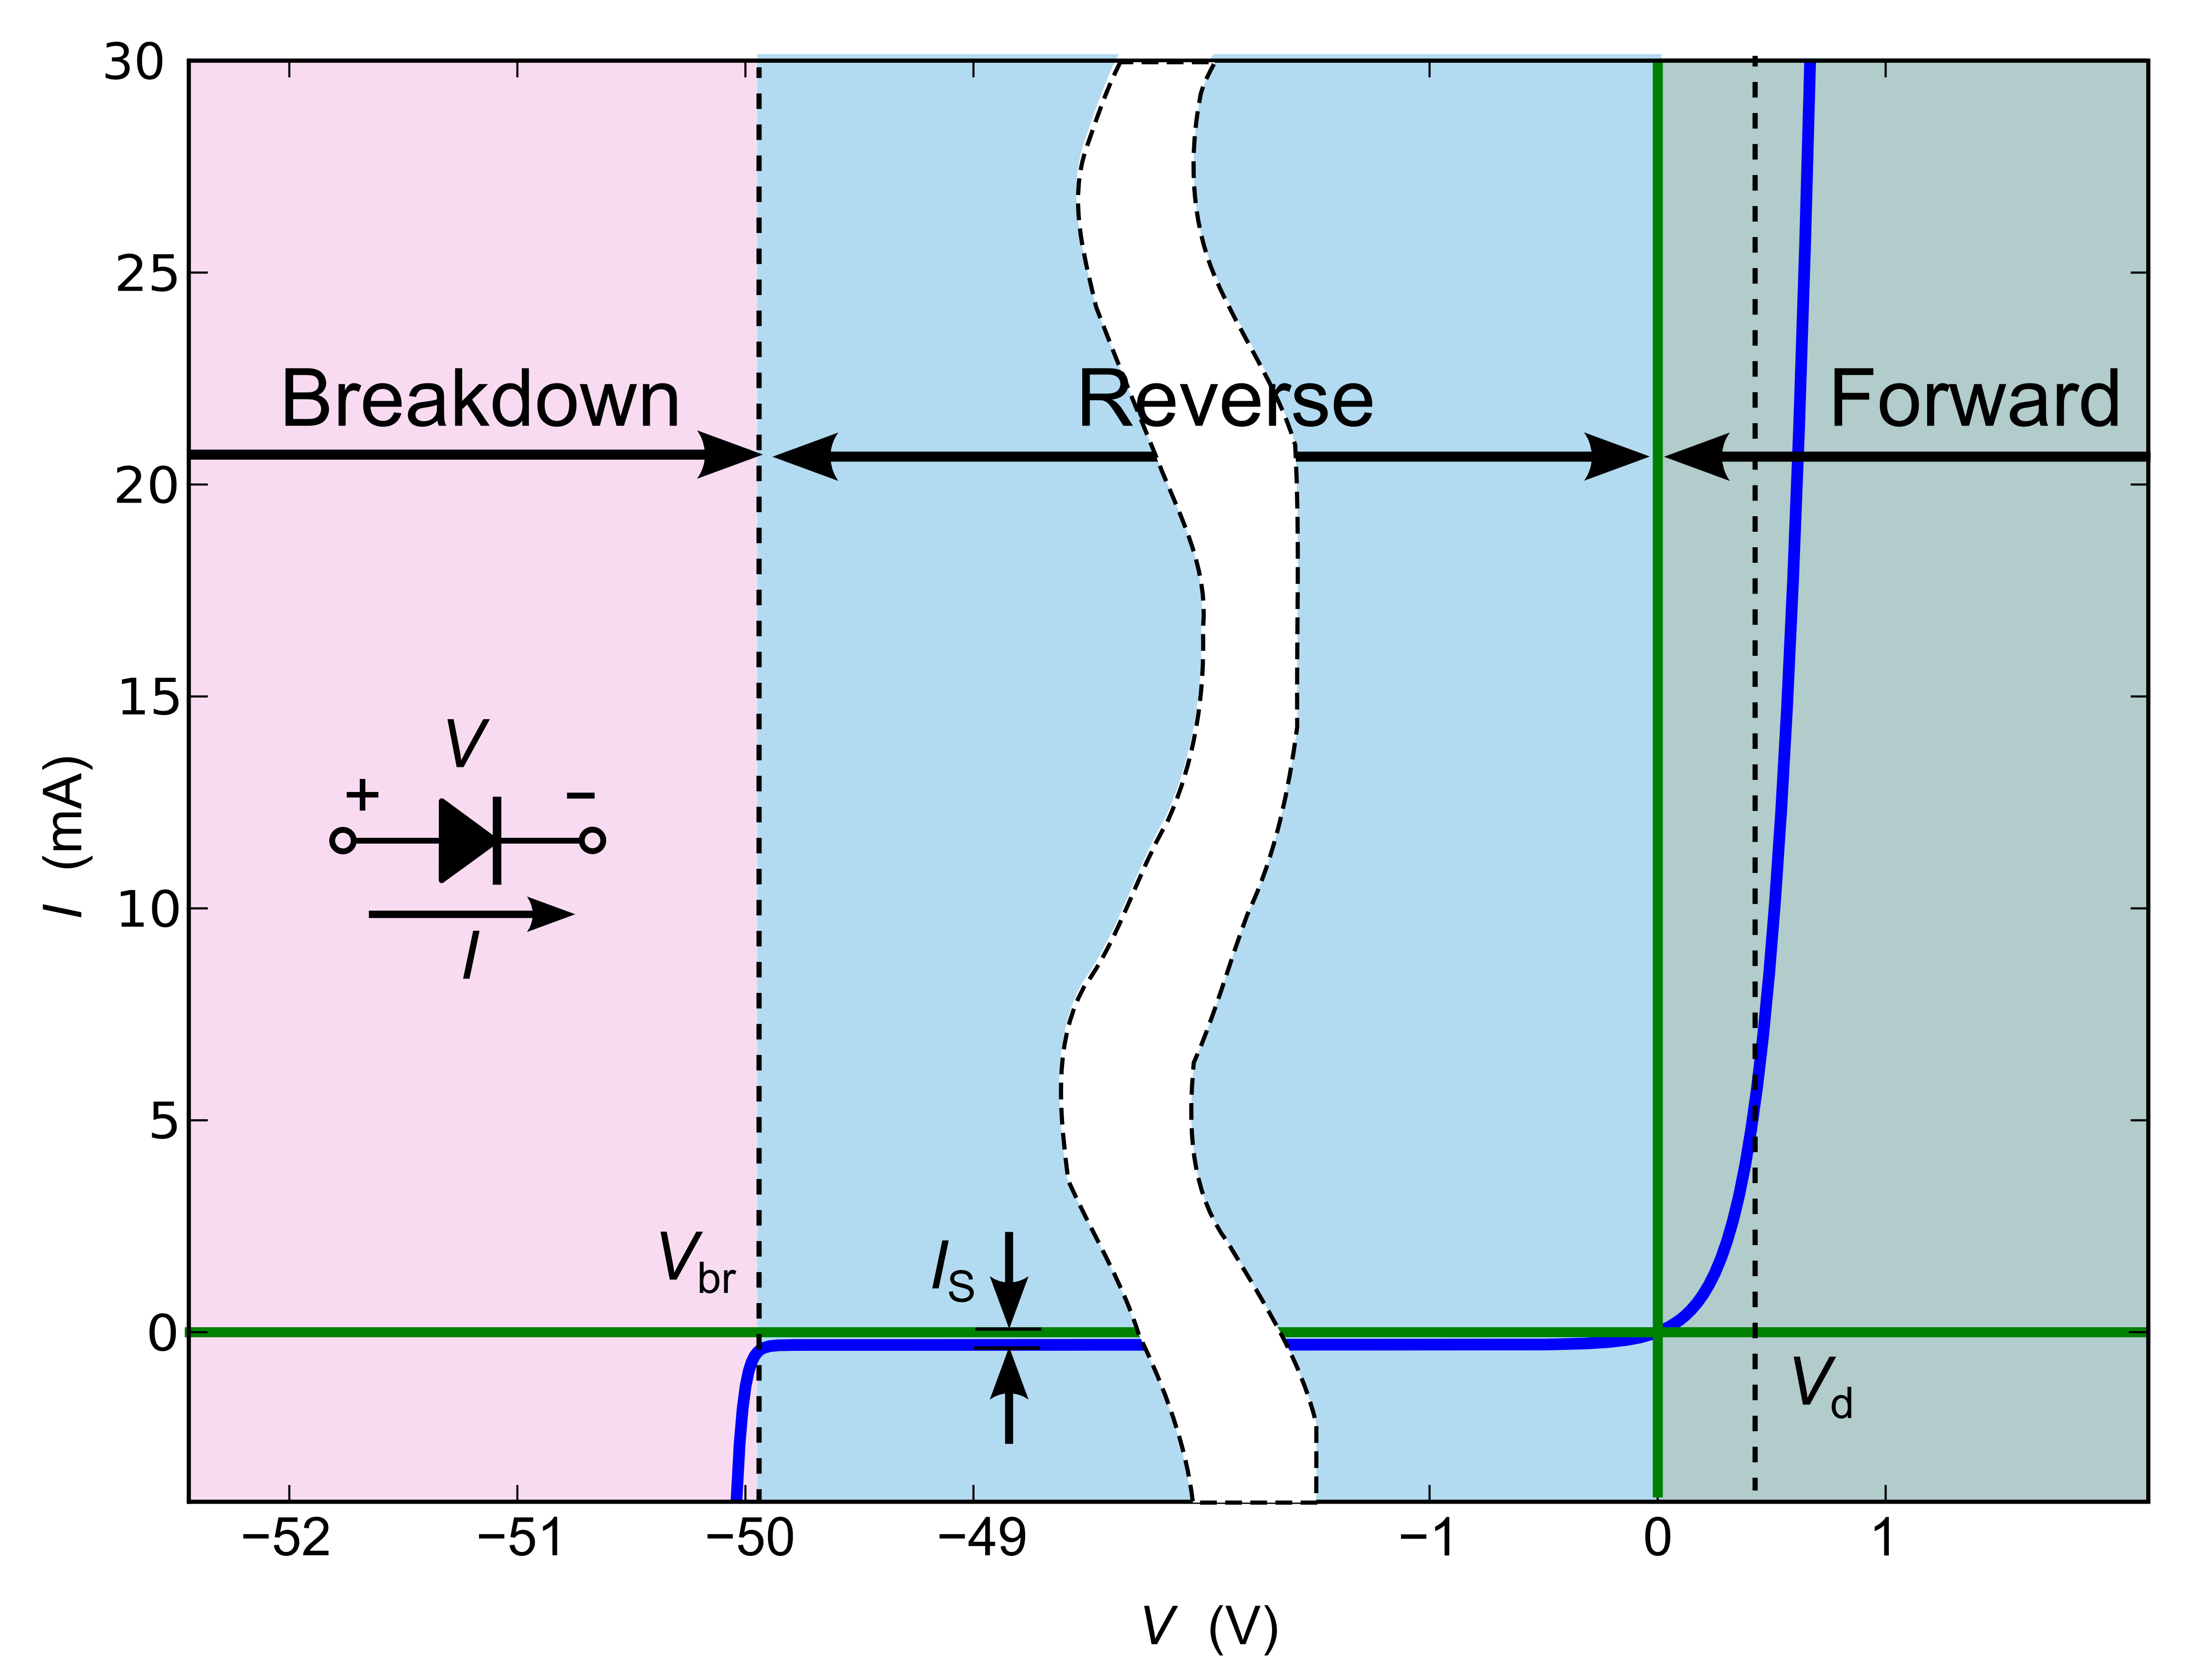
\includegraphics[width=10cm]{lab6fig/diode-characteristics.png}
    \caption{ \href{https://commons.wikimedia.org/wiki/File:Diode_current_wiki.png}{Diode characteristics}}
    \label{diode-char}
\end{figure}

A diode is a semiconductor device that has two terminals, an anode and a
cathode. These terminals are represented by (-) for the cathode and (+)
for the anode on the diagram in Figure \ref{diode-char}. Diodes are made out
of n-doped and p-doped semiconductors. For a good example of how these
work, see: \href{https://phet.colorado.edu/en/simulation/semiconductor}{https://phet.colorado.edu/en/simulation/semiconductor}

The fundamental property of a diode is its tendency to conduct electric
current in only one direction. The diode can be operated in three
regions. The first region, called forward biased, is when the cathode
has a higher potential relative to the anode. Once this potential
difference is greater than some threshold voltage (about 0.6
V for silicon diodes) the diode conducts with almost zero resistance and
has a constant 0.6 V drop across it. The second region of operation is
where the cathode has a lower potential relative to the anode. This
region is called reversed biased and essentially no current can flow.
Finally, if the potential difference from the cathode to the anode is
negative and larger than some breakdown voltage, the diode will again
conduct. Regular diodes are not used in the break down region, but Zener
diodes are used for this purpose.

\subsection{Light emitting diode (LED)}

The HLMP-C625 light emitting diode used in this lab acts electrically like any other diode. However, unlike regular diodes it also emits light when forward-biased due to direct radiative recombination of electrons and holes. The forward voltage drop is about 1.9 V rather than 0.6 V because the LED is made of AlInGaP instead of silicon.  

\subsection{Photodiode}

\begin{figure}
    \centering
    
\includegraphics{tmp}
    \caption{Diagram and schematic symbol for a PIN silicon photodiode.}
    \label{photodiode}
\end{figure}

The PD204 photodiode used in this experiment is a p-intrinsic-n (PIN) silicon diode operated in reverse bias. A
sketch of the photodiode structure is shown in Figure \ref{photodiode}. The very thin p-type conducting layer acts as a window to
admit light into the crystal. The reverse bias voltage maintains a strong electric field throughout the intrinsic
region forming an extended depletion layer. The depletion layer should be thicker than the absorption length
for photons in silicon in order to maximize the efficiency. An incident photon whose energy exceeds the bandgap energy can be absorbed to produce an electron-hole pair by photoelectric excitation of a valence electron
into the conduction band. The charge carriers are swept out of the crystal by the internal electric field to appear
as a photocurrent at the terminals. The photocurrent is proportional to light intensity over a range of more than
6 orders of magnitude.

The photodiode sensitivity $S_{\lambda}$ is the proportionality factor that links how incident optical power $P$ in Watts to a
generated current $I$ in Amperes. The photodiode sensitivity $S_{\lambda}$ carries units of A/W.

$$I=S_{\lambda}P$$

It is important to keep in mind that here, Amperes is the current flowing in the electrical circuit, whereas Watts
refers to the incident optical power, NOT an electrical power somewhere in the circuit.

What would $S_{\lambda}$ be for an ideal photodiode in which every photon hitting the photodiode
generates one electron? Since each photon of light at wavelength $\lambda$ carries an energy $E_{\lambda}=hc/\lambda$, the
rate of photons hitting the photodiode is $R=P/E_{\lambda}$ photons/second. But for an ideal photodiode,
every photon generates one electron with charge $e$ that then flows out of the photodiode. Therefore,
the rate of charge flowing out of the photodiode per second (i.e. the current!) is $I=eR=P~(\lambda e)/(hc)$. However, in a real photodiode, not every photon gets absorbed and generates an electron. We call
the probability that an incident photon at wavelength $\lambda$ generates an electron, the quantum efficiency
of the photodiode $q_{\lambda}$ with possible values between 0 and 1 such that $S_{\lambda}\le q_{\lambda}~(\lambda e)/(hc)$. At $\lambda$ = 690 nm (red), the ideal sensitivity (i.e. $q_{\lambda}= 1$) would be 0.56 A/W, a fairly easy number to remember.

The quantum efficiency also depends on $\lambda$, so photodiode manufacturers typically will provide the actual $S_{\lambda}$ in
the data sheet. Because the PD204 photodiode comes with a curved lens, the data sheet specifies the short
circuit current $I_{SC} = 10 ~\mu A$ at an incident intensity of $1 ~mW/cm^2$ at $\lambda$ = 940 nm. The lens has a diameter of $d = 0.3 ~cm$ or an area of 0.071 $cm^2$. So, an incident intensity of $1 ~mW/cm^2$ corresponds to a total power of
71 $\mu W$ of optical power hitting the photodiode. The sensitivity is then:

$$S_{940} = \frac{I_{SC}}{71~\mu W} = 0.14~A/W$$

Note that this means the quantum efficiency at 940 nm is only 0.18, not so great.

The sensitivity at other wavelengths $\lambda$ is given on the data sheet in terms of the peak sensitivity $S_{940}$ at 940 nm
times a correction factor called the relative spectral response, or RSR:

$$S_{\lambda} = S_{940}~RSR(\lambda)$$

Figure \ref{pd204} shows the RSR from the PD204 data sheet. You can see the maximum sensitivity is around 940 nm.

\begin{figure}[h]
    \centering
    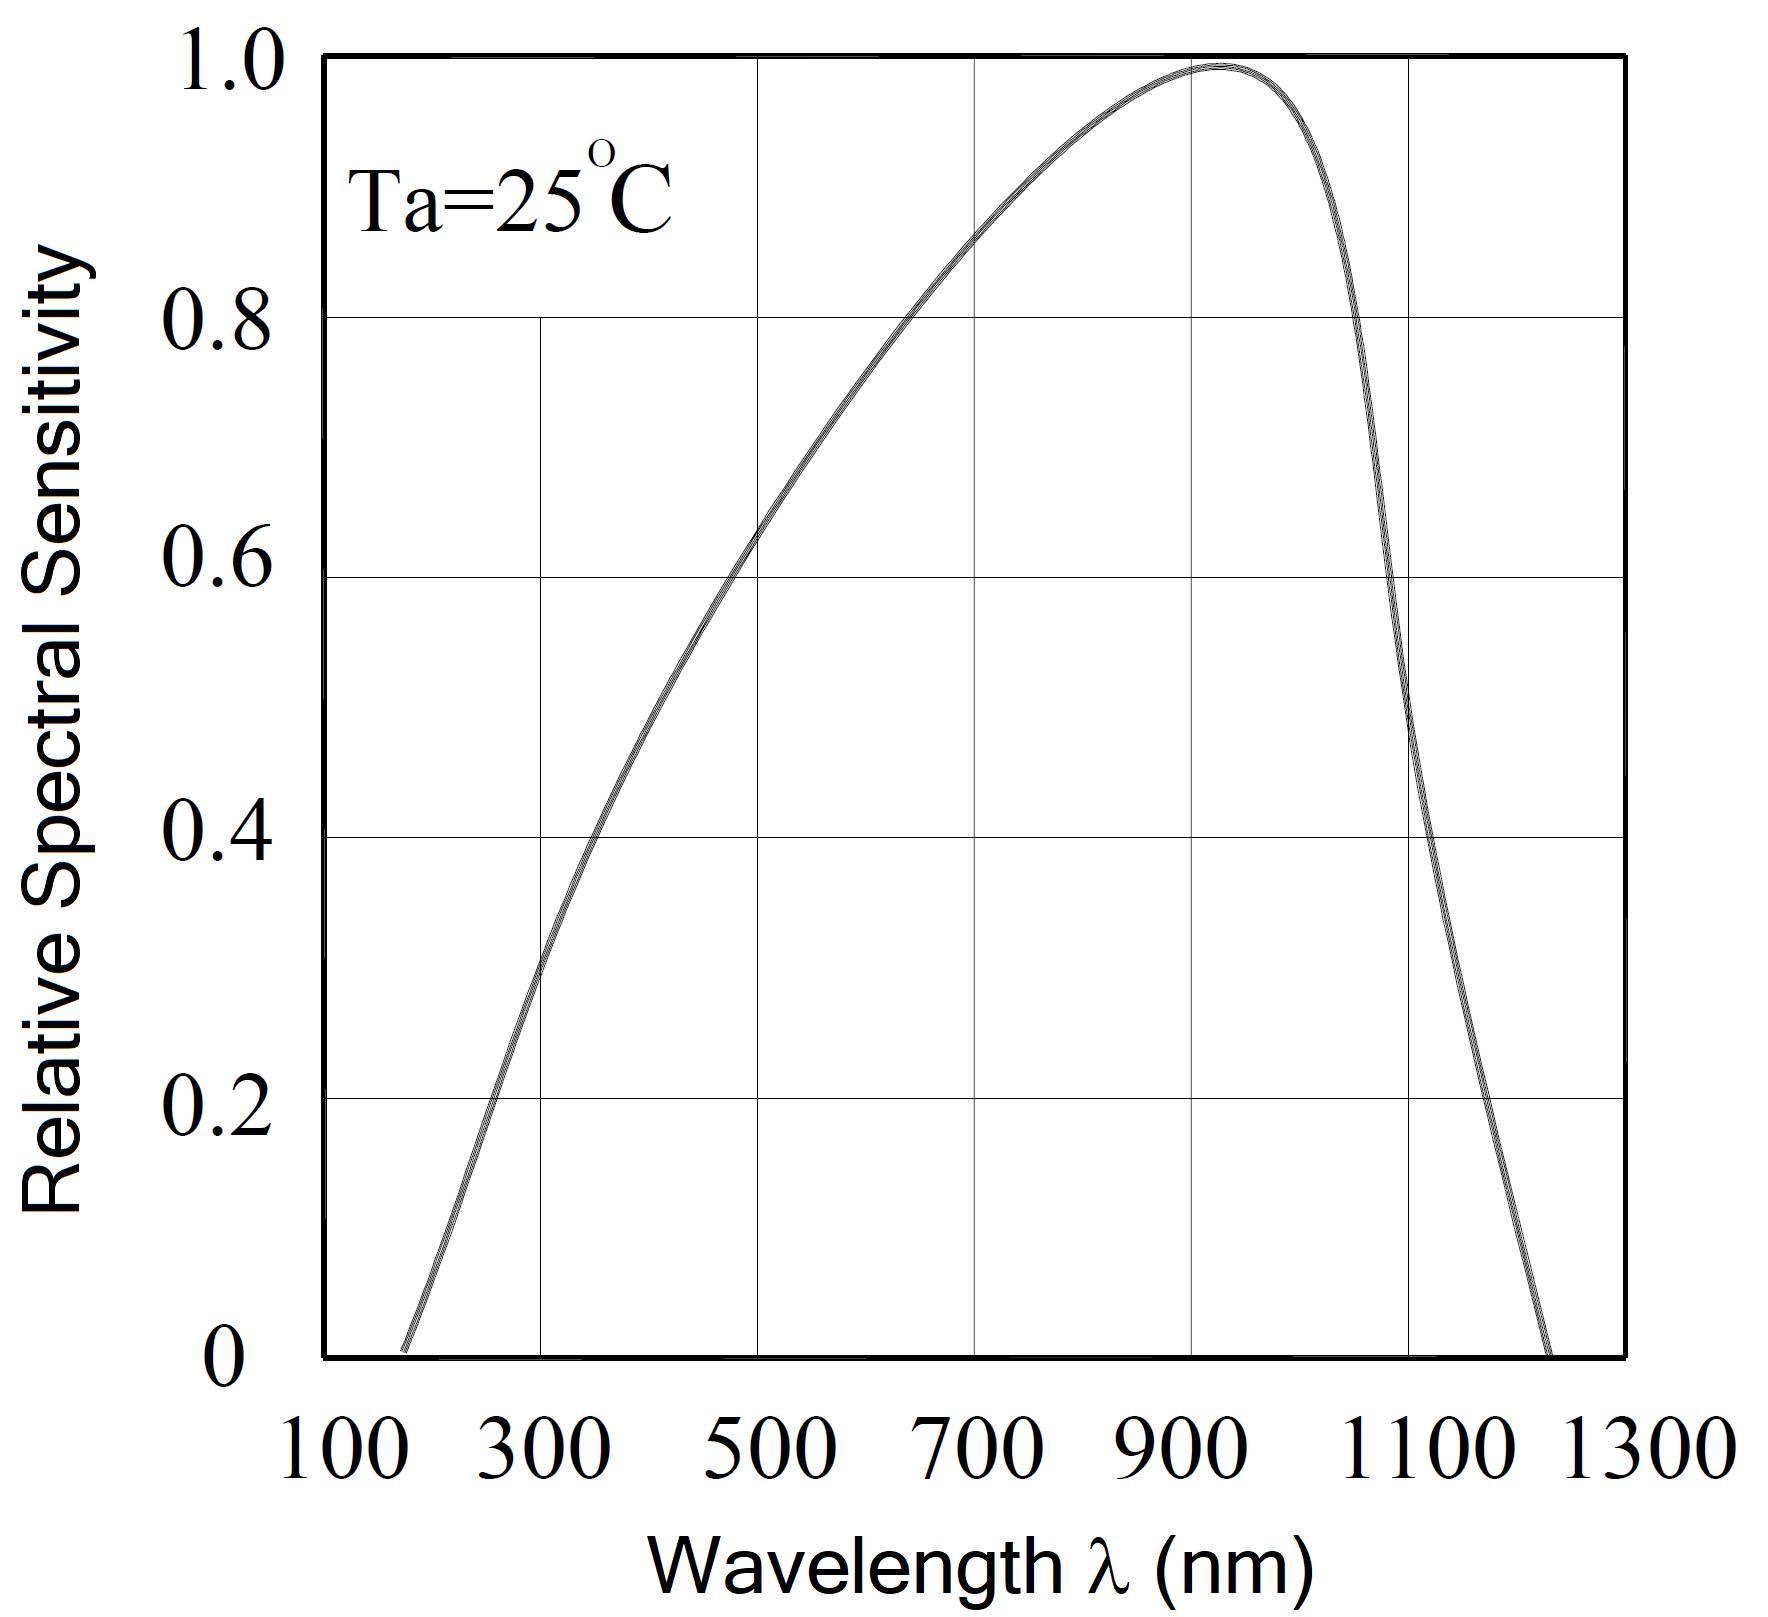
\includegraphics[width=7cm]{lab6fig/pd204-rss.png}
    \medskip
    \caption{PD204 Relative Spectral Sensitivity}
    \label{pd204}
\end{figure}
%------------------------------------------------

\section{Current to Voltage Amplifier (Transimpedance Amplifier)}

In an ordinary inverting amplifier, the input voltage is applied to a resistor, and the amplifier generates an output
voltage in response to the current that flows through the input resistor to the virtual ground at the negative op-amp input. A current-to-voltage amplifier (Figure \ref{photodetector}) is an inverting amplifier with the input current $I_{in}$ supplied by
the photodiode and applied to the inverting op-amp input. Since no current flows into the op-amp input, the
output voltage must be $V_{out} = –I_{in}R_F$. The ideal (Golden Rules result) low-frequency gain of a current-to-voltage
amplifier is

$$G=\frac{V_{out}}{I_{in}}=-R_F$$

This gain has the units of impedance i.e., Ohms, and it is often called a transimpedance gain. The current-tovoltage amplifier is also called a transimpedance amplifier. This type of amplifier is very common in research
labs, and is used to amplify the current from photodiodes, photo multiplier tubes, ion detectors, etc.

\begin{figure}[h]
    \centering
    \begin{circuitikz}[american voltages]
    \draw (0,0) node[op amp, anchor=-](OA){\texttt{}} 
    (OA.+) -- ++(0,0) node[ground]{}
    (OA.down) to [short, -o] ++(0,-1) node[anchor = north]{$-15~V$}
    (OA.down) to [short, -*] ++(0,-.5) to [C] ++(2,0) node[ground]{}
    (OA.up) to [short, -o] ++(0,1) node[anchor = south]{$+15~V$}
    (OA.up) to [short, -*] ++(0,.5) to [C] ++(2,0) node[ground]{}
    (OA.out) -- ++(1.25,0) coordinate(FC) to [short, -o] ++(1,0) node[anchor = west]{$V_{out}$}
    (OA.-) to [short, -*] ++(0,0) to [short, -*] ++(0,2) to [R, l=$R_F$] ++(4,0) to [short,*-*] ++(0,-2.5)
    (OA.-) -- ++(0,0) to ++(0,3.5) to [C, l=$C_F$] ++(4,0) to ++(0,-2.5)
    (OA.-) -- ++(-2,0) to [pD, invert, mirror, l=PD204] ++(0,-2) to [short, -o] ++(0,0) node[anchor = north]{$-15~V$}
    ;
    \end{circuitikz}
    \caption{Photodetector circuit}
    \label{photodetector}
\end{figure}

In our photometer circuit the current $I_{in}$ flows through the reverse-biased photodiode when it is
illuminated (it flows out of the op-amp negative input node and the resulting $V_{out}$ is positive). The feedback
capacitor $C_F$ enhances stability, i.e., it helps to avoid spontaneous oscillations of the op-amp by reducing the
bandwidth of the amplifier (just like an active low-pass filter).

%------------------------------------------------

\section{Optical Communication Link}

The basic optical communication link is composed of two circuits (Figure \ref{photodetector} and Figure \ref{ocl}). The circuit in Figure \ref{ocl} uses an AC voltage source to produce a light signal from the LED. The circuit in Figure \ref{photodetector} is the photometer,
composed of a photodiode connected to a transimpedance amplifier to convert the light into a measurable
voltage.

\begin{figure}[h]
    \centering
    \begin{circuitikz}[american voltages]
    \draw (0,0) to [short, o-] (0,0)  node[anchor = east]{$V_{in}$} to (1,0) to [R,l=$R_s$] ++(0,-2) to [short, -*] ++(0,0) to ++(1,0) to [pD,l=HLMP-C625] ++(0,-2) to ++(-1,0) node[ground]{} to ++(-1,0) to [D,l=$1N4002$] ++(0,2) to ++(1,0)
    ;
    \end{circuitikz}
    \caption{Optical communication link circuits}
    \label{ocl}
\end{figure}

%------------------------------------------------

\section{LF356 Pin Out and Schematic}

All op-amp circuits start out by making the basic power connections. Op-amps are active components, which
means they need external power to function, unlike passive components such as resistors and capacitors.

\begin{figure}[h]
 \centering
 \begin{circuitikz}[american voltages]
    \draw (0, 0) node[op amp] (opamp) {};
    \draw (opamp.-) node[above right]{2} node[anchor = east]{$V_-$};
    \draw (opamp.+) node[above right]{3} node[anchor = east]{$V_+$};
    \draw (opamp.out) node [above left]{6} node[anchor = west]{$V_{out}$};
    \draw (opamp.up) node[above right]{7} to (-.08,1.25) node[anchor = south]{$+15~V$};
    \draw (opamp.down) node[below right]{4} to (-0.08,-1.25) node[anchor = north]{$-15~V$};
    \path (2.5,0.75) node[dipchip, anchor=pin 1, num pins=8]{LF356};
 \end{circuitikz}
 \caption{LF356 schematic and pin-out.}
  \label{lf356}
\end{figure}

%------------------------------------------------

\section{Useful Readings}

\begin{enumerate}
\item
  \href{https://atomoptics-nas.uoregon.edu/~dsteck/teaching/electronics/electronics-notes.pdf}{Steck}
  Sections 2.2.1, 3.1, 3.3, 3.4, 3.6, Problem 7.5 (pages 246-246)
\item
  Fischer-Cripps Chapter 4, especially Sections 4.18-4.19
\item
  Horowitz and Hill 2\textsuperscript{nd} Ed., Sections 1.25-1.27, 15.02, and page 184
\end{enumerate}

%------------------------------------------------

\section{Prelab}

Answer the following questions using Mathematica for the plots. You can use either Mathematica for the rest
of the questions as well or do them by hand. \textbf{Make sure to have the Mathematica notebook for your lab
section as well.}

\subsection{Simple diodes}

\label{simp-diodes}

\begin{enumerate}
    \item Consider the circuit in Figure \ref{diode-cir}. If the diode is ideal with a threshold voltage of 0.6 V and a
breakdown voltage of 50 V, predict the behavior of the current $I$ (consider clockwise
current to be positive) and $V_{out}$ as a function of the source voltage $V_{in}$. Make a table of
the predicted $I$ and $V_{out}$ for the following values of $V_{in}$: -2 V, 0 V, +0.5 V, +0.6 V, +0.7 V, +1 V, +2 V, +4 V.
\item Now, consider the case where $V_{in}$ is a sine wave with a 3 V amplitude (6 V peak-to-peak)
centered on $V_{in}$ = 0 V. Predict $V_{out}$ and $I$ as a function of time and sketch your predictions
(by hand or with Mathematica) over 3 periods.
\end{enumerate}

\subsection{Transimpedance amplifier}

\label{trans-pre}

\begin{enumerate}
    \item 
    For the current-to-voltage amplifier in Figure \ref{photodetector}, choose a value for the feedback resistor $R_F$
so that an incident white-light ($\lambda$ = 555 nm) optical power of P = 71 $\mu$W produces an
output of 10 V.
\item 
The small feedback capacitor $C_F$ is used to suppress spontaneous oscillations. The transimpedance gain of the amplifier at any particular frequency is $–Z_F$, where $Z_F$ is the effective
impedance of the parallel $R_FC_F$ circuit. The gain rolls off at high frequencies with a
bandwidth of $f_B = 1/(2\pi R_FC_F)$, just like any low-pass filter. The bandwidth will suffer if $C_F$ is
too large. What is the bandwidth $f_B$ if $C_F$ = 10 pF?
\item
What are the DC values of the voltages at the + and – inputs and at the output of the op-amp for zero light on the photodiode? Consider the ideal situation where the diode allows
zero current when there is no light hitting it. (In reality, about 10 nA of “dark current”
flows through the diode even with no light on it.)
\end{enumerate}

\subsection{Optical Communication Link}

\begin{enumerate}
    \item 
    To drive the transmitter, the function generator will be adjusted to produce a square
wave with a high level of 8 V (unloaded) and a low level of 0 V. The high-level (8 V) should
give a 20 mA forward current in the LED, and the low level (0 V) should give 0 mA. \textbf{Find
the value of the series resistor Rs that gives the correct current. }The data sheet lists the
LED forward voltage drop at 20 mA to be 1.9 V (instead of 0.6 V for silicon diodes). In
addition, do not forget to model the function generator as an ideal voltage supply with a
series output impedance of 50 $\Omega$, which is the true output impedance regardless of the
“impedance setting” on the function generator. You will want to draw a circuit diagram
with all of the components (modeling the output impedance as an extra resistor) and then
use Kirchoff’s rules to generate an equation that you can solve for $R_S$.
\end{enumerate}


\subsection{Lab activities}

\begin{enumerate}
\item
  Read through all of the lab steps and identify the step (or sub-step)
  that you think will be the most challenging.
\item
  List at least one question you have about the lab activity.
\end{enumerate}

%------------------------------------------------

\section{Introducing Diodes}

\begin{figure}[h]
    \centering
    \begin{circuitikz}[american voltages]
    \draw (0,0)
        to [V, invert, l=$V_{in}$] (0,4)
        to [rmeter, t=A] ++(2,0) to [R, l=$33~\Omega$] ++(0,-2) coordinate(FB) 
        to [D,l=$1N4002$] ++(0,-2) to ++(-1,0) node[ground]{} to (0,0);
    \draw (FB) to [short, *-] ++(0,0) to [short, -o] ++(1,0) node[anchor = west]{$V_{out}$}  
    ;
    \end{circuitikz}
    \caption{Simple diode circuit}
    \label{diode-cir}
\end{figure}

\subsection{Determine the I-V characteristics for a silicon diode}

\label{iv-silicon}

\begin{enumerate}
    \item 
    Build the circuit in Figure \ref{diode-cir} using the silicon diode 1N4002.
    \item 
     Measure the current $I$ and the voltage across the diode ($V_{out}$) for different values of $V_{in}$
from –3 V to +3 V. You need to use the DMM to measure the voltage across the diode.
To maximize accuracy, you would use another DMM to measure current. But reading
the current directly from the power supply is fine. Be sure to take many data points (at
least 10) to map out the characteristic curve of the diode, with a few extra points
around $V_{in}$ of 0.6–0.9 V. How does the result compare with your predictions from
section \ref{simp-diodes}.1? How does it compare with Figure \ref{diode-char}?   
    \item 
           Specifically consider the points at $V_{in}$ = +0.5 V, +0.8 V, and +2.0 V. What is the power
dissipated in the diode and in the resistor for these values? Remember $P = IV$ and $I$ is the
same for both components, but $V$ is not. 
    \item 
    Now, change $V_{in}$ from the DC voltage source (power supply) to the AC voltage source
(function generator) and input a 1 kHz sine wave with a 3 V amplitude (6 V peak-to-peak) Record the resulting $V_{out}$ waveform and compare with your prediction in section \ref{simp-diodes}.2.
\end{enumerate}

\subsection{Determine the I-V characteristics for a light emitting diode}

\begin{enumerate}
    \item 
    Now, replace the silicon diode with a red LED (HLMPC625). Repeat section \ref{iv-silicon}.2, but take the
extra points in the region where the current begins to rapidly increase. Be sure to read
the spec sheet for the LED and don’t exceed the DC current limit. Take note whether the
LED is emitting light and give a qualitative description of the amount of light. How does
the LED behave differently in the circuit from a silicon diode? Does the LED’s light output
seem to be proportional to voltage or current, or some combination?
\end{enumerate}
%------------------------------------------------

\section{Test with Inverting Amplifier}

\begin{figure}[h]
    \centering
    \begin{circuitikz}[american voltages]
    \draw (0,0) node[op amp, anchor=-](OA){\texttt{}} 
    (OA.+) -- ++(0,0) node[ground]{}
    (OA.down) to [short, -o] ++(0,-1) node[anchor = north]{$-15~V$}
    (OA.down) to [short, -*] ++(0,-.5) to [C] ++(2,0) node[ground]{}
    (OA.up) to [short, -o] ++(0,1) node[anchor = south]{$+15~V$}
    (OA.up) to [short, -*] ++(0,.5) to [C] ++(2,0) node[ground]{}
    (OA.out) -- ++(1.25,0) coordinate(FC) to [short, -o] ++(2,0) node[anchor = west]{$V_{out}$}
    (OA.-) to [short, -*] ++(0,0) to [short, -*] ++(0,2) to [R, l=$R_F$] ++(4,0) to [short,*-*] ++(0,-2.5)
    (OA.-) -- ++(0,0) to ++(0,3.5) to [C, l=$C_F$] ++(4,0) to ++(0,-2.5)
    (OA.-) to [R, l=$R$] ++(-3,-0) to [short, -o] ++(0,0) node[anchor = east]{$V_{in}$}
    ;
    \end{circuitikz}
    \caption{Inverting amplifier circuit}
    \label{inv-amp-cir}
\end{figure}

\begin{enumerate}
    \item 
    We will first build the amplifier in a normal voltage amplifier configuration to test the
setup and all the connections. Build the inverting amplifier circuit shown in Figure \ref{inv-amp-cir}. Use
a value for $R_F = R$ close to what you found in \ref{trans-pre}, and a 10 pF capacitor $C_F$
in parallel with the feedback resistor to avoid spontaneous oscillations. Draw the
schematic in your lab notebook and record the values of the components.
\item
 Predict the low frequency gain and 3 dB frequency of the circuit. HINT: Look at your
prelab answers. This will be the $R_FC_F$ time constant from \ref{trans-pre}; in this circuit the
time constant will be determined by the feedback resistor and capacitor (not the input
resistor). Design a test to ensure the amplifier is working as predicted at low frequency
(much lower than the cutoff). Don’t bother testing the high-frequency behavior.
\end{enumerate}

%------------------------------------------------

\section{Room Light Photometer}

\begin{enumerate}
    \item 
    Reconfigure your voltage amplifier to the transimpedance amplifier circuit shown in Figure \ref{photodetector}. Pay attention to the direction of the photodiode. You can use your DMM set to the
“diode setting” to determine which side of the diode is the cathode.
\item
Verify that it changes as a function of the amount of incident light on the photodiode,
for instance, by putting your hand over the photodiode to shade it from the room lights.
\end{enumerate}
%------------------------------------------------

\section{Optical Communication Link}

\subsection{LED emitter}

\begin{enumerate}
    \item 
    Set up a light emitting diode type HLMP-C625 as the transmitter on a separate small
circuit board according to the schematic in Figure \ref{ocl}  (!!!!). Be sure to protect the LED with
a series resistance that prevents the forward current exceeding 20 mA. HINT: You
calculated the required resistance in the prelab. Also, the LEDs have a nominal
breakdown voltage of 5 V, which, if exceeded, can damage the LED. Therefore, to
prevent this from happening, connect a regular diode in parallel with the LED but with
opposite polarity. This will protect the LED from a large negative voltage.
    \item
    Set up the function generator to produce 5 Hz square waves with the low voltage level
0 V and the high voltage of 8 V. You can accomplish this by using the DC offset setting
of the function generator. Connect this to the oscilloscope and the LED circuit. Make
sure the oscilloscope shows a square wave that goes from 0 V to 8 V and that you see
the LED flashing 5 times per second before moving on.
\end{enumerate}

\subsection{Measure the output of the LED with the photometer}

\begin{enumerate}
    \item 
    Place the LED transmitter close to the photodiode and verify that the photodiode sees
the light from the LED. The LED is directed forward so make sure to orient both the LED
and photodiode so they are pointing at each other to maximize the amount of light
detected. You can bend the wire leads to get both devices pointed horizontally. You
can check the alignment by using a piece of white paper to see if the red illumination is
centered on the photodiode.
    \item
    Observe the input driving signal and the output of the receiver on the scope using DC
coupling for both signals. Make sure the received signal is due to the red LED, and not
from an electrical connection. How did you determine that it was working? You may
want to increase the frequency to about 100 Hz to allow the scope to update faster. You can
also try switching to AC coupling for the receiver to see if it is easier to see the signal.
    \item
    Determine the frequency limitations of your photometer. We did this in previous labs
by measuring the frequency dependence of sine waves to find where the gain dropped
by 3 dB. This method is only correct for sine waves. For square waves, we can use
another method. A low-pass filter in the time domain is an integrator. This means it
charges or discharges exponentially with a time constant of $RC$. Measure the time it
takes for the signal to rise from the base level (room lights) to $(1–1/e)$ of the maximum
value or to fall from the maximum value to $1/e$ of the difference between the maximum
value and the base level. This gives the time constant $RC$. As the 3 dB frequency is $f_B =1/2\pi RC$, you can determine $f_B$. Does this measurement agree with your model
predictions?
    \item
    Measure the output of the transimpedance amplifier (in Volts) of the transmitted light
versus distance from a few cm to about 0.5 meter. How does the background light from
the room affect the signal? Explain how you made this measurement. Estimate the
the photodiode sensitivity $S_{\lambda}$ at the wavelength 625 nm of light emitted by the LED. Plot
the power in Watts hitting the photodiode as a function of distance.
\end{enumerate}

%------------------------------------------------

\section{Summary and Conclusions}

Write a two-paragraph summary in your lab notebook of what you learned
and any important takeaways.

%------------------------------------------------

\section*{Appendix A: Some Related Concepts About Measuring Light}

\addcontentsline{toc}{section}{Appendix A: Some Related Concepts About Measuring Light} % Adds this section to the table of contents

The sun has a power output (radiant flux) of $P = 3.85~x~10^{26}$ watts. Assuming a transparent atmosphere and a 1
m by 2 m solar panel perpendicular to the sun that absorbs 100\%  of the light, how much power is received?
Consider that the entire $3.85~x~10^{26}$ W is distributed evenly on a hypothetical sphere with radius $1.50~x~10^{11}$ m
(distance from sun to Earth). Since we know the area of a sphere is $4\pi r^2$, we can calculate the irradiance or
intensity (power per area) as $N = P/4\pi r^2 = 1360 W/m2$. Since the solar panel has an area of 2 $m^2$, the power
delivered to the solar panel is 2720 W.

There are additional concepts and units that are made necessary by the fact that the eye is not uniformly
sensitive to all wavelengths and we are often interested in how humans perceive things. The luminous flux is
measured in units of lumens (lm) and is basically the same as the power (measured in watts) except that the
spectrum of emitted light is weighted by the eye’s response. The conversion from radiant flux (power) in watts
to luminous flux in lumens is given by:

$$F(lm) = 683 ~y(\lambda)~P(W)$$

The dimensionless quantity $y(\lambda)$ is the photopic standard
luminosity function and is shown in Figure \ref{lum} and tabulated in the
Datasheets section of Canvas. At $\lambda$ = 555 nm, where the eye is
most sensitive, $y(\lambda)$ = 1. Therefore, two sources with the same
luminous flux will have the same subjective brightness to a human
observer (even though the outputted power may be different).
This kind of color corrected unit is helpful if you want to design a
control panel with lots of colored lights, and you want them all to
have the same perceived brightness. We may also be interested
in the luminous flux per unit area (similar to intensity). This is
measured in units of lux, where 1 lux = 1 $lm/m^2$.

\begin{figure}
    \centering
    
\includegraphics{tmp.png}
    \caption{The photopic standard luminosity function}
    \label{lum}
\end{figure}

%------------------------------------------------


\section*{Appendix B: Light Output in Lumens for Various Light Sources}

\addcontentsline{toc}{section}{Appendix B: Light Output in Lumens for Various Light Sources} % Adds this section to the table of contents

%------------------------------------------------
\end{document}